\chapter{Evaluation}\label{C:eval}

\section{Accuracy Testing}
\par To test the accuracy of the device, a loopback test was performed with different length of cables. This was 
setup so that there was no switch between two ethernet measurement ports, only an ethernet cable. The test is to 
ensure that the device is measuring the latency correctly, and able to detect the latency present in a specific 
length of cable. Latency measured from the device can be compared with the theoretical value of the latency which 
can be calculated using the following formula

\[Latency = \frac{L}{cV_f}\]

\par Where L is the length of the cable, c is the speed of light (299,792,458 m/s) and Vf is velocity factor of 
Ethernet Cables (0.65). 

\par A very short cable (4 cm) was used to measure the processing time, a constant added to every measurement. 
This processing time is the result of both Ethernet Phy’s converting between the two protocols (Differential Pairs 
and RGMII). Performing measurements with the short cable produced a mean value of 440 ns. 

\par This processing time is then removed from subsequent tests, making the latency values produced by the device 
purely the latency present in the cable.

\begin{figure}[H]
    \begin{center}
        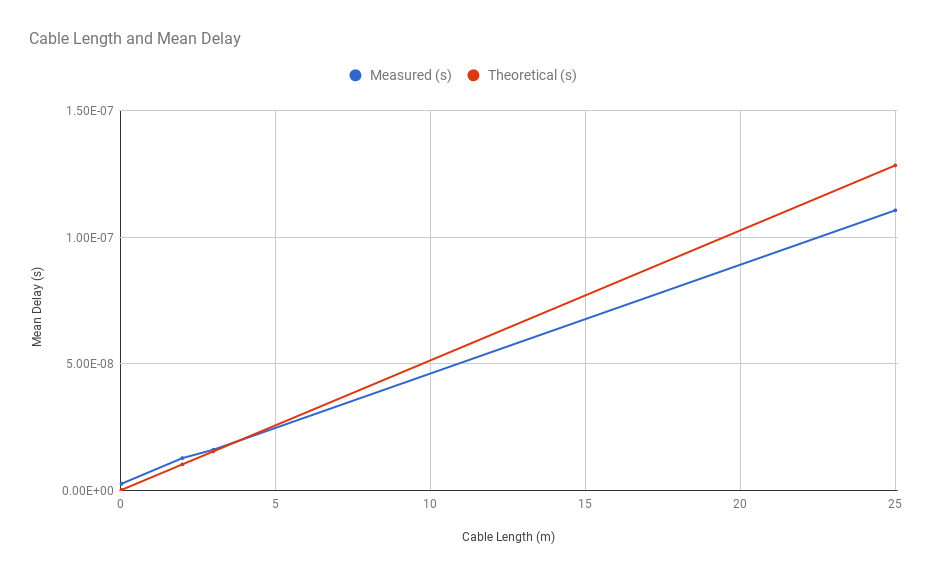
\includegraphics[keepaspectratio,width=15cm]{Images/CableTesting}
        \caption{Results from Accuracy Measurements}
        \label{fig:accuracyMeasurements}
    \end{center}
\end{figure}

\par As shown in ~\ref{fig:accuracyMeasurements}, the results from the device show a linear trend in latency due to 
length of the cable. These offset of the theoretical line can be attributed to the fluctuation in velocity factor 
through the different cables.

\section{Reliable Testing}
